\chapter{Funzionalità dell'utente}
In questo capitolo verranno descritte più in dettaglio le funzionalità relative alle azioni dell'utente nella scena finale, in modo che si possa comprendere meglio il lato progettuale dietro il loro effettivo funzionamento nella scena.
\\È utile, innanzitutto, ricordate che sono state ideate due tipologie di utenti: 
\begin{itemize}
    \item Docente (\textit{Master Client}): gode di particolari privilegi ed è abilitato all'uso di tutte le funzionalità, tranne la \textit{Richiesta di Parlare} (\ref{Request});
    \item Studente (\textit{Generic Client}): non gode di alcun privilegio ed è abilitato all'uso di alcune funzionalità.
\end{itemize}
\section{XR Origin}
Prima di procedere con la descrizione delle funzionalità vere e proprie, è necessario fare una descrizione dell'oggetto che in ogni progetto in Realtà Virtuale non può mancare: \textbf{XR Origin}.
\begin{figure}[H]
    \centering
    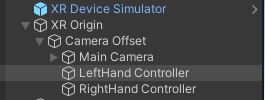
\includegraphics[scale = 1]{Immagini/XROrigin.jpg}
    \caption{XR Origin nella Hierarchy del progetto}
    \label{fig:4.1}
\end{figure}
\hspace{-0.6cm}La presenza di questo oggetto all'interno del progetto è vitale, perché senza esso gli utenti non possono in alcun modo muoversi nell'ambiente, compiere qualsiasi tipo di azione o visualizzare la scena nel proprio visore. 
\\Nella \textbf{Figura \ref{fig:4.1}} è rappresentato XR Origin con le sue componenti:
\begin{itemize}
    \item \textit{Main Camera}: l'oggetto che permette la visualizzazione della scena all'utente;
    \item \textit{LeftHand Controller}: l'oggetto che rappresenta il \textit{controller} sinistro nella scena
    \item \textit{RightHand Controller}: l'oggetto che rappresenta il \textit{controller} destro nella scena
\end{itemize}
\begin{figure}[H]
    \centering
    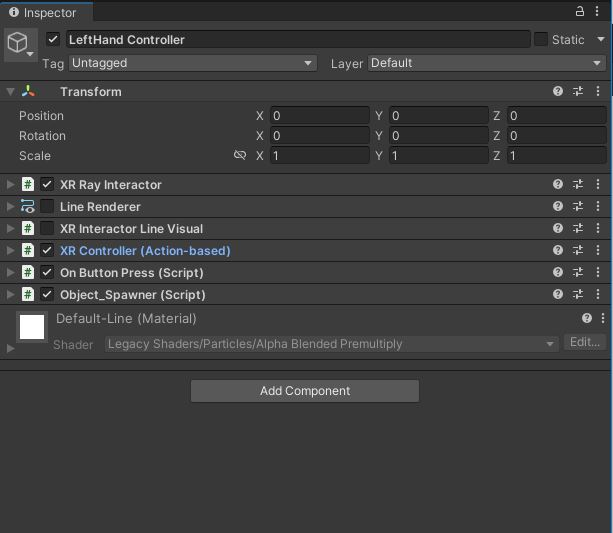
\includegraphics[scale = 0.8]{Immagini/InspectorXRcontroller.jpg}
    \caption{Componenti del LeftHand Controller}
    \label{fig:4.2}
\end{figure}
Nella \textbf{Figura \ref{fig:4.2}} sono illustrate le componenti che abilitano il \textit{controller} sinistro (\textit{LeftHand Controller}) allo svolgimento di determinate azioni.
\\Per esempio, le componenti \textit{XR Ray Interactor, Line Render, XR Interactor Line Visual} si occupano della renderizzazione grafica di un raggio e dell'interazione che ha quest'ultimo con gli oggetti in scena, mentre \textit{XR Controller} è la componente che si occupa di tracciare i vari input che provengono dal \textit{controller} sinistro, quali il movimento lungo i tre assi cardinali e la pressione di uno specifico tasto.
\\Ovviamente le componenti appena elencate, se applicate all'oggetto \textit{RightHand Controller}, hanno l'effetto analogo sul \textit{controller} destro.
\section{Creazione e distruzione di oggetti}
Questa funzionalità è stata progettata per poter permettere al docente di manipolare l'ambiente tramite la creazione e distruzione di oggetti (\textbf{bandierine}) in determinati punti della scena (\textbf{pannelli}).
\\Abbiamo pensato che questa funzione possa essere utile per segnare luoghi particolari all'interno della scena e renderli, così, più visibili alla vista degli utenti.
\begin{figure}[H]
    \centering
    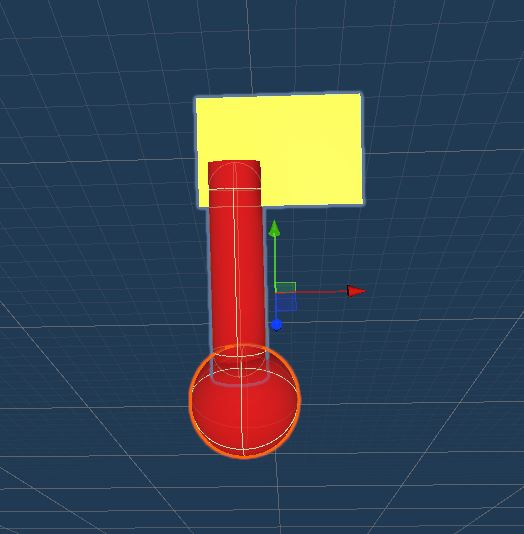
\includegraphics[scale = 0.4]{Immagini/bandierina.jpg}
    \caption{Modello della bandierina che viene creata all'interno della scena}
    \label{fig:my_label}
\end{figure}
\hspace{-0.6cm}Sulla bandierina e sui pannelli sono sono applicati gli script C\# \textit{Photon View} e \textit{Photon Transform View} della libreria \textit{Photon.Pun} che permettono la visualizzazione degli oggetti a tutti gli utenti in scena.
\begin{figure}[H]
    \centering
    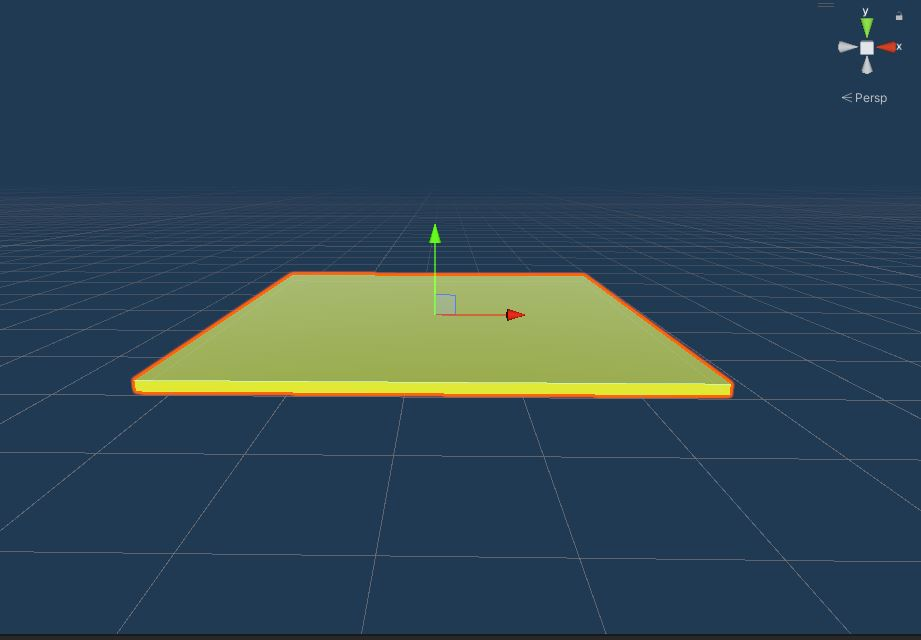
\includegraphics[scale = 0.4]{Immagini/pannello.jpg}
    \caption{Modello del pannello su cui vengono create le bandierine}
    \label{fig:my_label}
\end{figure}
\hspace{-0.6cm}Inoltre, i pannelli possiedono una componente \textit{Conta Bandiere} che tiene traccia del numero delle bandiere sul pannello.
\subsection{Object\_Spawner}
\textit{Object\_Spawner} è la classe C\# che permette al docente di creare le bandierine in scena.\\Questa componente è applicata all'oggetto \textit{LeftHand Controller}, per cui le bandierine potranno essere create esclusivamente tramite l'utilizzo del \textit{controller} sinistro.
\begin{figure}[H]
    \centering
    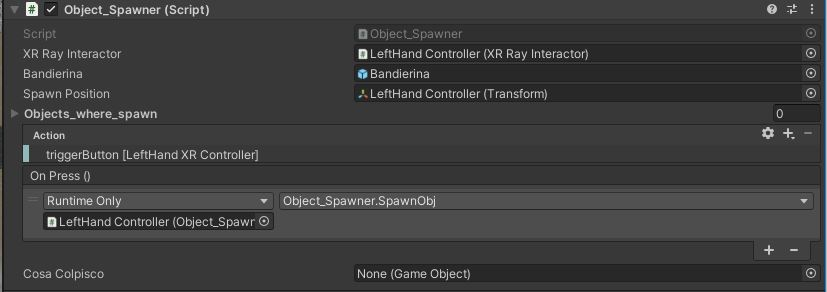
\includegraphics[width = 16cm, height = 7cm]{Immagini/Object_spawner.jpg}
    \caption{Object\_Spawner in dettaglio}
    \label{fig:4.5}
\end{figure}
\hspace{-0.6cm}Nella \textbf{Figura \ref{fig:4.5}} sono illustrati i campi pubblici della classe \textit{Object\_Spawner} nell'\textit{Inspector Panel} di Unity.
\\Dall'alto verso il basso troviamo:
\begin{itemize}
    \item \textbf{XR Ray Interactor}: il raggio del \textit{controller} (nel nostro caso verrà impostato il raggio sinistro);
    \item \textbf{Bandierina}: il modello della bandierina che si vuole creare;
    \item \textbf{Spawn Posizion}: il punto di collisione tra il raggio e un oggetto in scena;
    \item \textbf{Objects\_where\_spawn}: lista di oggetti (pannelli) su cui le bandierine possono essere create;
    \item \textbf{Action}: il comando sul \textit{controller} sinistro (in questo caso il tasto \textit{triggerButton}) che permette di eseguire il metodo indicato nella sezione \textit{On Press()} (il metodo \textit{SpawnObj()});
    \item \textbf{Cosa Colpisco}: l'oggetto con cui interseca il raggio del \textit{controller} sinistro.
\end{itemize}
L'abilitazione dell'azione, cioè il tasto sul \textit{controller}, è gestita nel metodo \textit{Update()} della classe \textit{Object\_Spawner}, in seguito verrà mostrato il diagramma di flusso che mostra le condizioni in cui l'azione è abilitata o no.
\begin{figure}[H]
    \centering
    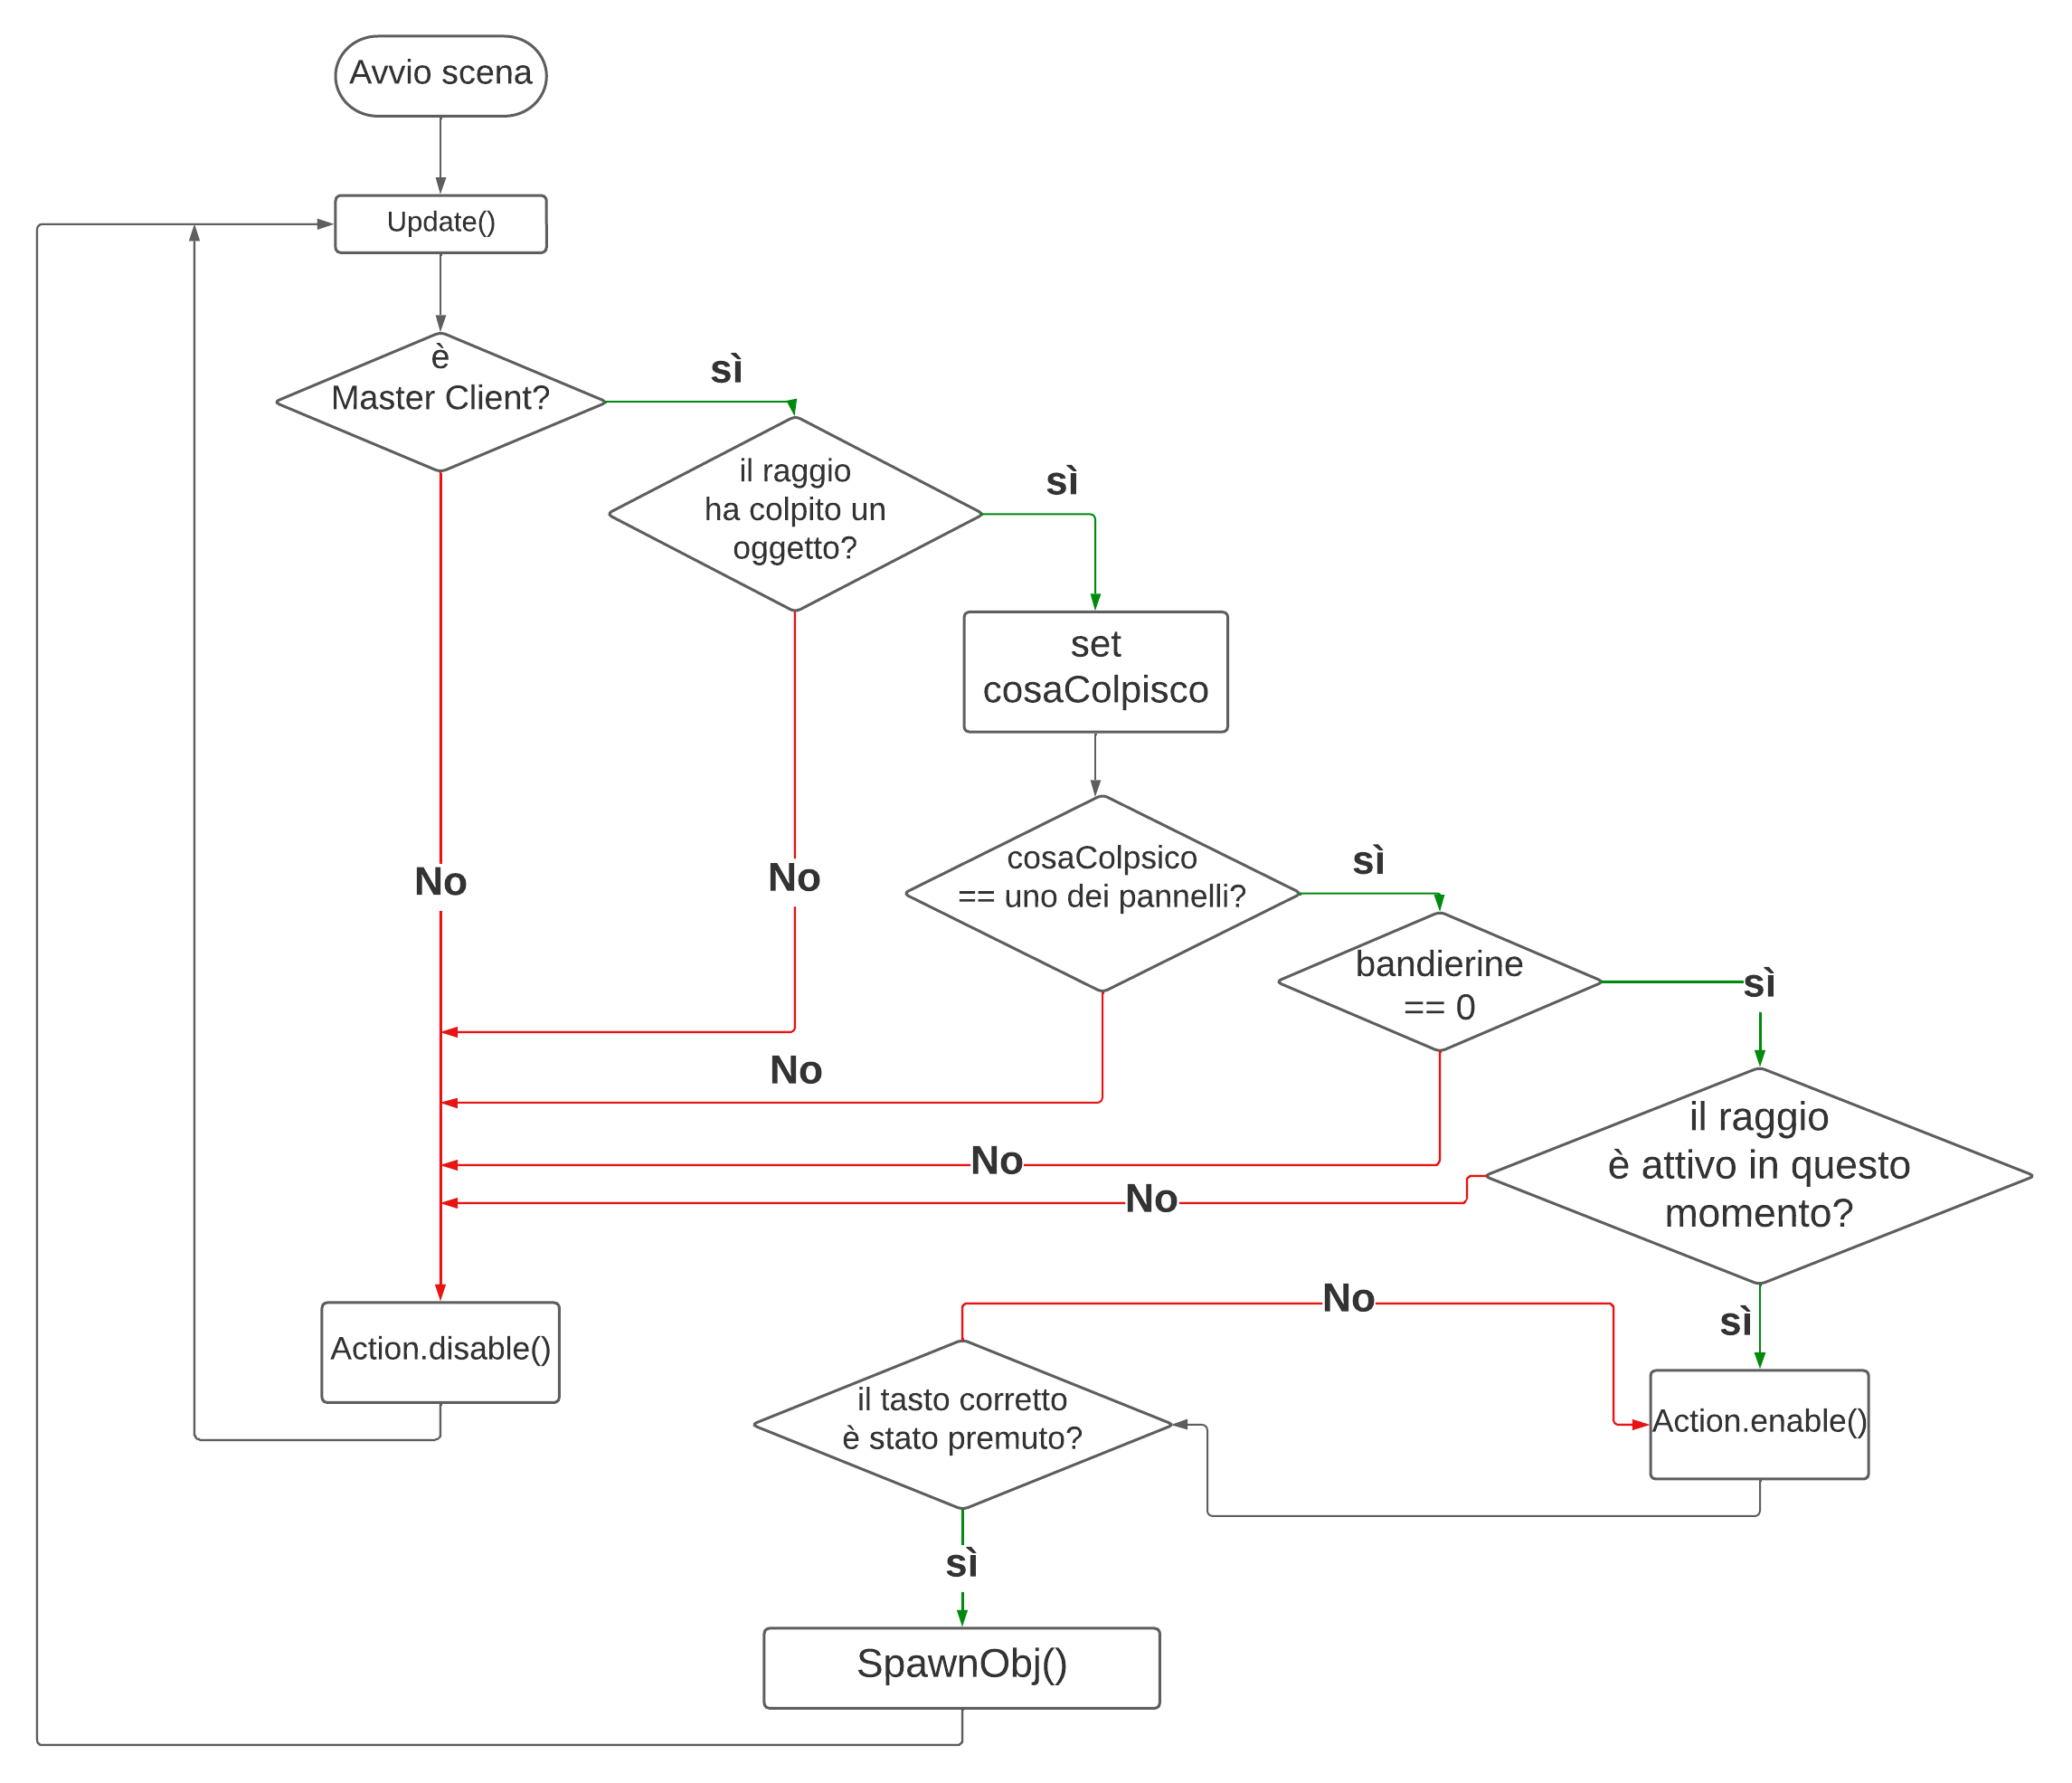
\includegraphics[scale = 0.45]{Immagini/Diagramma SpawnObj().jpg}
    \caption{Diagramma di flusso del metodo Update() della classe Object\_Spawner}
    \label{fig:4.6}
\end{figure}
\hspace{-0.6cm}Il metodo \textit{Update()} viene eseguito costantemente durante l'esecuzione dell'applicazione, perciò le condizioni mostrate nella \textbf{Figura \ref{fig:4.6}} vengono controllate di continuo.
\subsection{Object\_Destroyer}
\textit{Object\_Destroyer} è la classe C\# che permette al docente di distruggere le bandierine in scena.\\Questa componente è applicata all'oggetto \textit{Bandierina} e le bandierine potranno essere distrutte esclusivamente tramite l'utilizzo del \textit{controller} sinistro.
\begin{figure}[H]
    \centering
    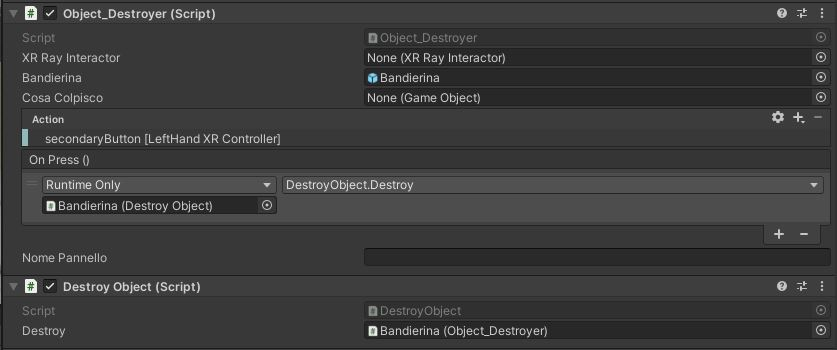
\includegraphics[scale = 0.7]{Immagini/Object_destoryer.jpg}
    \caption{Object\_Destroyer e DestroyObject in dettaglio}
    \label{fig:4.7}
\end{figure}
\hspace{-0.6cm}Nella \textbf{Figura \ref{fig:4.7}} sono illustrati i campi pubblici della classe \textit{Object\_Destroyer} nell'\textit{Inspector Panel} di Unity.
\\Dall'alto verso il basso troviamo:
\begin{itemize}
    \item \textbf{XR Ray Interactor}: raggio del \textit{controller} (nel nostro caso verrà impostato il raggio sinistro);
    \item \textbf{Bandierina}: il modello della bandierina che si vuole distruggere;
    \item \textbf{Cosa Colpisco}: l'oggetto con cui interseca il raggio del \textit{controller} sinistro;
    \item \textbf{Action}: il comando sul \textit{controller} sinistro (in questo caso il tasto \textit{secondaryButton}) che permette di eseguire il metodo indicato nella sezione \textit{On Press()} (il metodo \textit{DestroyObject.Destroy}));
    \item \textbf{Nome Pannello}: il nome del pannello su cui la bandierina viene creata;
\end{itemize}
L'abilitazione dell'azione, cioè il tasto sul \textit{controller}, è gestita nel metodo \textit{Update()} della classe \textit{Object\_Destroyer}, in seguito verrà mostrato il diagramma di flusso che mostra le condizioni in cui l'azione è abilitata o no.
\begin{figure}[H]
    \centering
    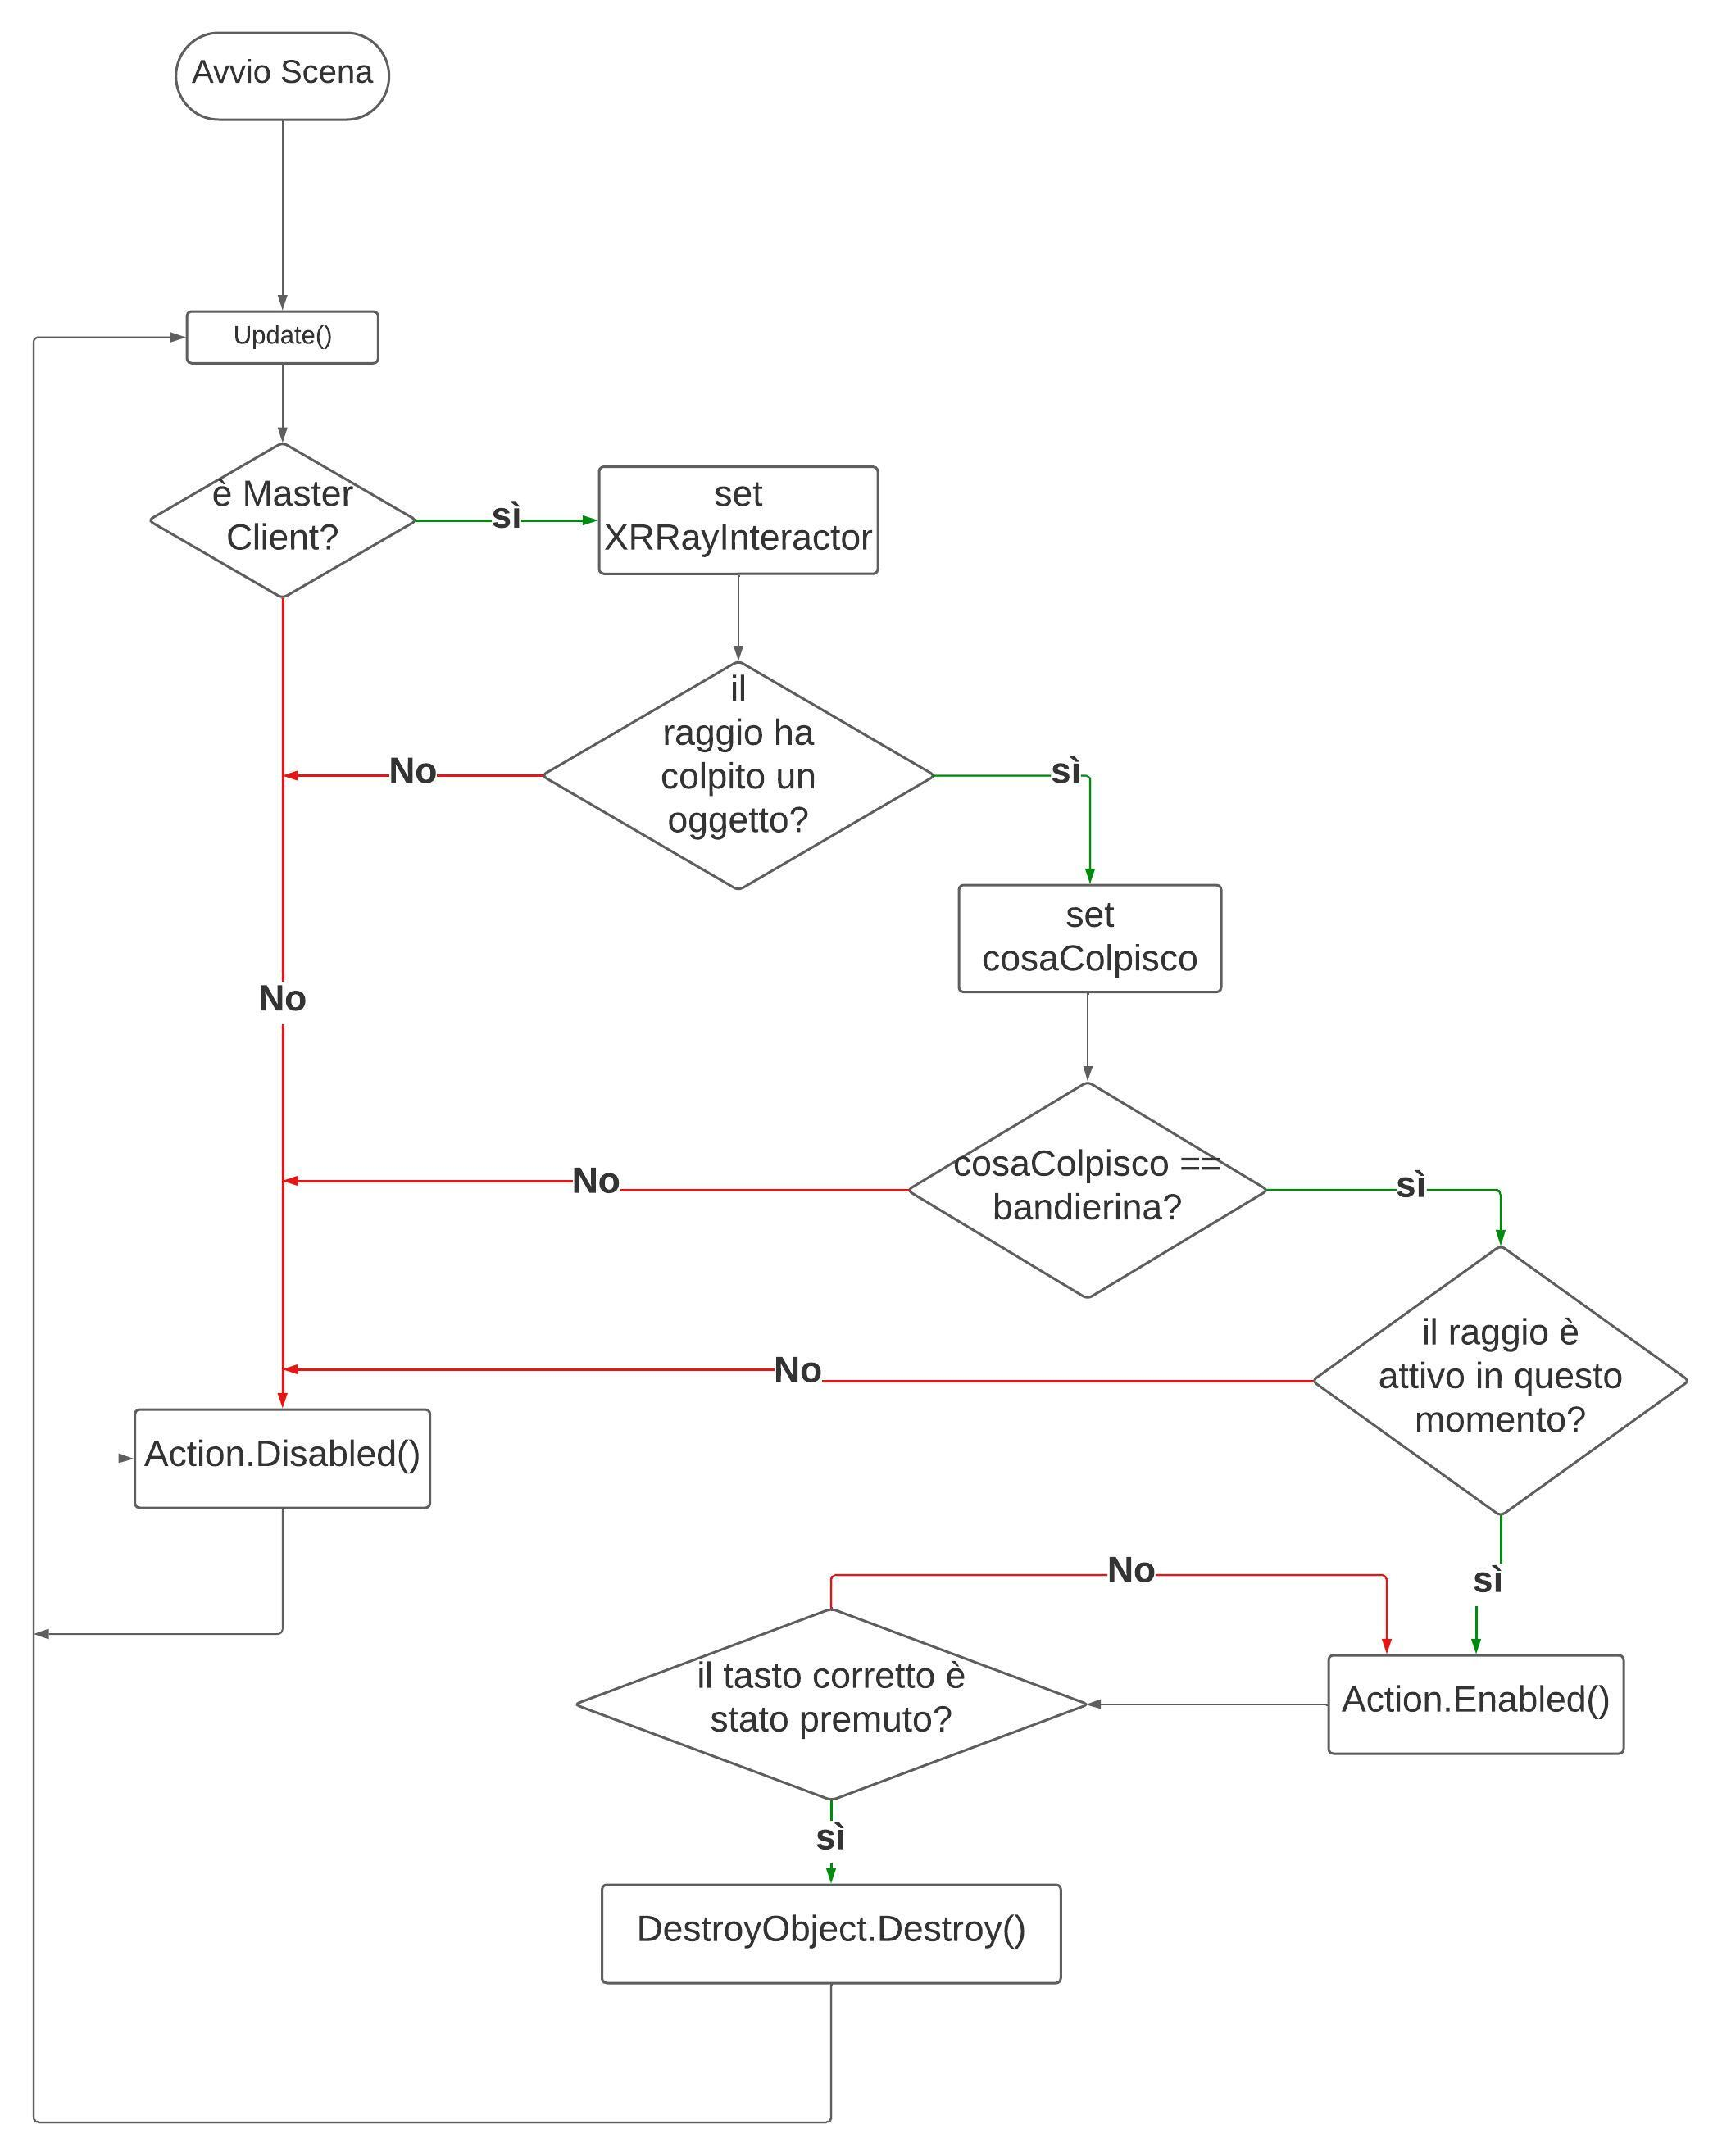
\includegraphics[scale = 0.45]{Immagini/ObjectDestroyer().jpg}
    \caption{Diagramma di flusso del metodo Update() della classe Object\_Destroyer}
    \label{fig:4.8}
\end{figure}
\hspace{-0.6cm}Anche in questo caso, il metodo \textit{Update()} viene eseguito costantemente durante l'esecuzione dell'applicazione, perciò le condizioni mostrate nella \textbf{Figura \ref{fig:4.8}} vengono controllate di continuo.
\\La differenza rispetto al caso della creazione delle bandierine, è che il metodo abilitato appartiene ad una classe esterna.
\\Per concludere, si può notare che le funzionalità appena descritte sono delegate ai comandi del \textit{controller} sinistro, questa scelta è stata effettuata sia per una comodità d'uso, per un utente potrebbe risultare scomodo utilizzare una funzionalità sul \textit{controller} sinistro e una sul \textit{controller} destro, sia in ottica sviluppi futuri, applicare le stesse funzionalità ad entrambi i \textit{controller} costringe lo sviluppatore a toglierle da un \textit{controller} prima di poterne applicare altre.
\section{Unity Canvas e Interfaccia Utente}
Le funzionalità che verranno illustrate in seguito sono relative all'interfaccia utente, che viene realizzata con gli oggetti \textbf{Unity Canvas}.
\\Il Canvas è un oggetto di gioco che possiede una componente \textit{Canvas} e tutti gli elementi dell'interfaccia utente devono essere figli di tale Canvas.
\\L'area del Canvas viene mostrata come un rettangolo nella scena, ciò permette una maggiore semplicità nel posizionamento degli elementi dell'interfaccia utente.
\\Gli elementi dell'interfaccia utente sono di vario tipo, ad esempio componenti visuali (come testo e immagini) e componenti interattive (come bottoni, barre di testo in cui è possibile scrivere, menù a tendina, barre di scorrimento e altro ancora).
\\Le componenti interattive sono attivabili tramite l'utilizzo di dispositivi di input, come ad esempio mouse, tastiera, \textit{controller} VR, microfono ecc...
\section{Chat interattiva}
Questa funzionalità è stata ideata per aggiungere un altro tipo di comunicazione tra utenti oltre a quella vocale.
\\L'interfaccia utente della chat è stata realizzata con gli oggetti \textbf{Unity Canvas}, in particolare è strutturata in 3 sezioni:
\begin{itemize}
    \item Join Room: Canvas che contiene il bottone per connettersi alla chat;
    \begin{figure}[H]
    \centering
    
\includegraphics[scale = 0.65]{Immagini/ChatBackground.jpg}
    \caption{Join Room Canvas}
    \label{fig:my_label}
    \end{figure}
    \newpage\item Chat Room: Canvas che rappresenta la chat vera e propria;
        \begin{figure}[H]
    \centering
    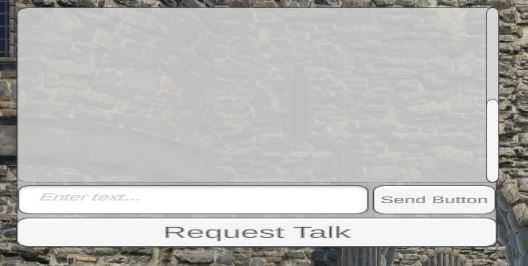
\includegraphics[scale = 1]{Immagini/ChatRoom.jpg}
    \caption{Chat Room Canvas}
    \label{fig:my_label}
\end{figure}
    Per inviare i messaggi è necessario innanzitutto scrivere, tramite la tastiera, nel campo con il testo \textit{`Enter text`}, e successivamente premere il bottone \textit{`Send Button`}.
    \\È presente anche un bottone (\textit{`Request Talk`}) per l'invio sulla chat di un messaggio prefabbricato, che lo studente può utilizzare qualora volesse richiedere l'attivazione del proprio microfono al docente. 
    \item Open Chat: Canvas con un apposito bottone che permette di aprire \textit{Chat Room}, è stato impostato un timer di 30 secondi che chiude \textit{Chat Room} se in quel lasso di tempo non sono arrivati messaggi sulla chat;
    \begin{figure}[H]
    \centering
    
\includegraphics[scale = 0.65]{Immagini/Openchat.jpg}
    \caption{Open Chat Canvas}
    \label{fig:my_label}
\end{figure}
\end{itemize}
Per comprendere meglio il funzionamento della chat, verranno ora illustrati i diagrammi di sequenza relativi alle 3 sezioni della chat mostrate in precedenza.
\\I diagrammi di sequenza illustrano come le diverse parti di un sistema interagiscono tra loro per svolgere una funzione, e l'ordine in cui le interazioni avvengono quando un particolare caso d'uso viene eseguito.
\\In parole più semplici, un diagramma di sequenza mostra diverse parti del lavoro di un sistema in una `sequenza` per ottenere qualcosa.
\begin{figure}[H]
    \centering
    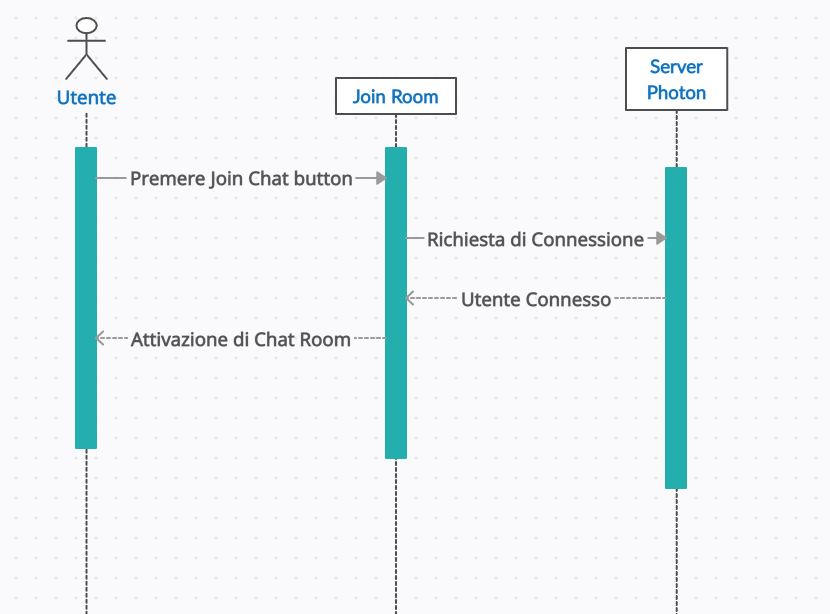
\includegraphics[scale = 0.65]{Immagini/ChatBackgrounddiagramma.jpg}
    \caption{Diagramma di sequenza per Join Room}
    \label{fig:my_label}
    \end{figure}
\begin{figure}[H]
    \centering
    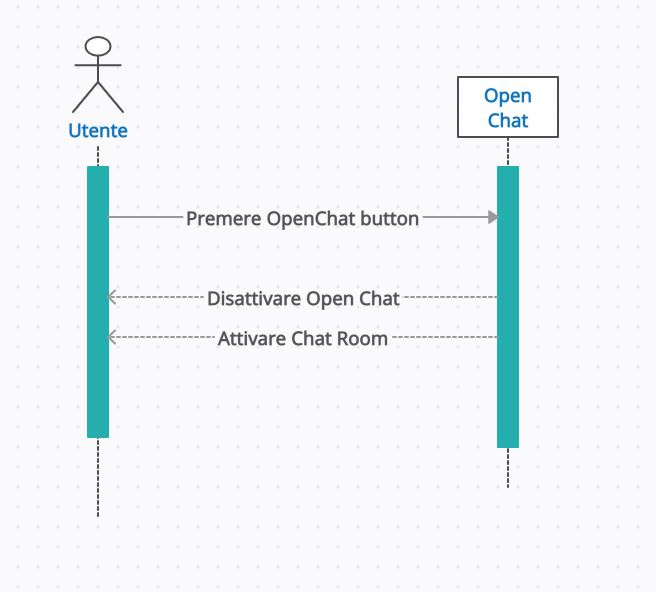
\includegraphics[scale = 0.65]{Immagini/Openchatdiagramma.jpg}
    \caption{Diagramma di sequenza per Open Chat}
    \label{fig:my_label}
\end{figure}    
\begin{figure}[H]
    \centering
    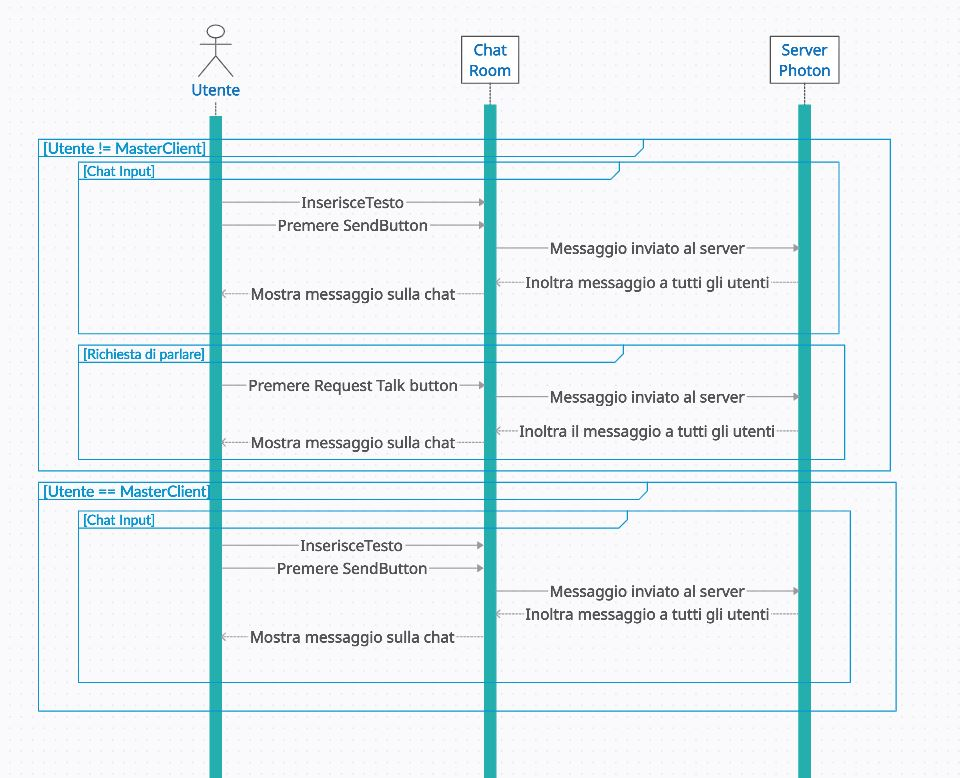
\includegraphics[width = 16cm, height = 16cm]{Immagini/ChatRoomddiagramma.jpg}
    \caption{Diagramma di sequenza per Chat Room}
    \label{fig:my_label}
    \end{figure}
\section{Abilitazione e disabilitazione audio utenti}
Questa funzionalità permette al docente di attivare e disattivare il microfono di tutti gli utenti presenti nella scena.
\\Anche in questo caso è presente un'interfaccia utente, realizzata con gli oggetti \textbf{Unity Canvas}, strutturata in due parti:
\begin{itemize}
    \item Apri Impostazioni: Canvas con un apposito bottone dedicato all'apertura della Schermata Utenti;
    \begin{figure}[H]
    \centering
    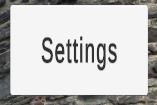
\includegraphics[scale = 1]{Immagini/settings.jpg}
    \caption{Apri Impostazioni Canvas}
    \label{fig:my_label}
\end{figure}
    \item Schermata Utenti: Canvas con la lista degli utenti connessi alla stanza con un bottone apposito per attivare o disattivare il microfono del giocatore desiderato.
    \begin{figure}[H]
    \centering
    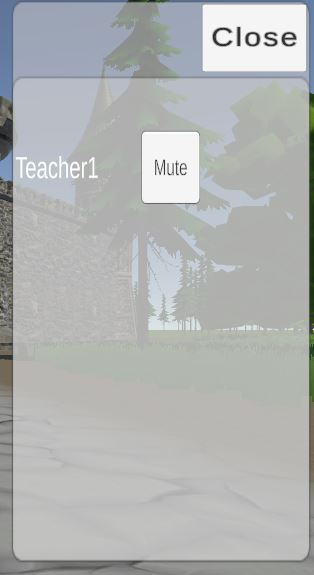
\includegraphics[scale = 1]{Immagini/MutareSmutare.jpg}
    \caption{Schermata Utenti Canvas}
    \label{fig:my_label}
\end{figure}
\end{itemize}
Anche in questo caso verrà illustrato il diagramma di sequenza per comprendere meglio il meccanismo di attivazione e disattivazione del microfono degli utenti.
    \begin{figure}[H]
    \centering
    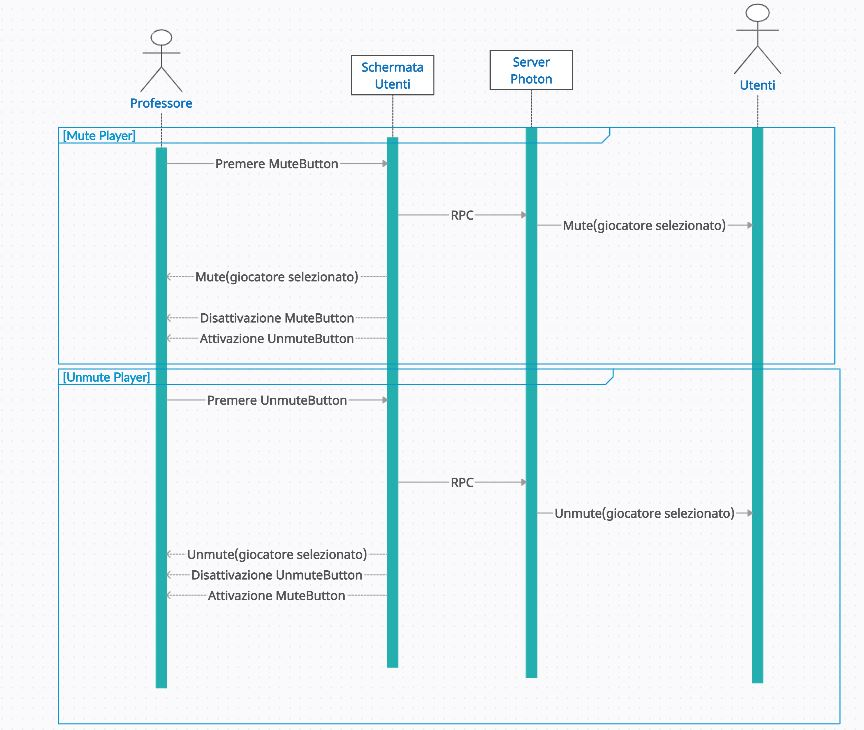
\includegraphics[width = 16cm, height = 16cm]{Immagini/muteunmutediag.jpg}
    \caption{Diagramma di sequenza per l'attivazione e disattivazione del microfono}
    \label{fig:my_label}
\end{figure}
\hspace{-0.6cm}Per sviluppare questa funzionalità è stato necessario ricorrere ad una particolare proprietà della libreria \textit{Photon.Pun}: le \textbf{RPC}.
\\Le chiamate di procedura remota (\textit{RPC}) sono il modo in cui \textit{Photon} esegue eventi o notifiche che si basano sul networking.
\\Impostando l'attributo RPC su un metodo, esso viene richiamato anche per gli altri utenti connessi alla rete \textit{Photon} o che si connetteranno in seguito.
\\In questo caso specifico, la chiamata di procedura remota è applicata al metodo che attiva o disattiva la componente microfono di un giocatore.